%!TEX root = paper_main.tex

\section{BLE Tracking Toolkit}
\label{sec:methodology}

In this section, we describe a toolkit to evaluate if an attacker can perform a
BLE tracking attack based on physical-layer fingerprinting. First, we describe
how BLE produces a similar physical-layer fingerprint to other wireless
protocols. Then, we describe the unique challenges of fingerprinting BLE
transmissions, and therefore why existing fingerprinting techniques do not work on BLE
transmissions. Next, we describe a new approach to fingerprinting BLE devices
using a novel joint imperfection estimation technique. Finally, we describe how
an attacker can use a sniffer to track a specific device by detecting if its
fingerprint matches one of the BLE devices nearby the sniffer.

\subsection{BLE has WiFi-like signal imperfections}


Physical layer fingerprinting relies on each BLE radio having unique hardware
imperfections introduced by manufacturing variations in its transmitter chain.
Different types of imperfections are introduced by different transmitter
architectures. Therefore, we need to understand the architecture of a typical BLE
chipset to understand what imperfections we need to fingerprint.

We investigated the architecture of several BLE chipsets used in popular mobile
devices, and found that WiFi and BLE are often integrated into the same device.
Also, internally, they share the same 2.4~GHz \iq frontend.
(Figure~\ref{fig:iq_arch}). This architecture, known as a ``combo chipset'' is
desirable for mobile devices because it reduces the device's overall size and
power consumption, and it serves as a point to synchronize both protocols'
2.4~GHz transmissions, so they do not interfere with each other.

\begin{figure}
    \centering
    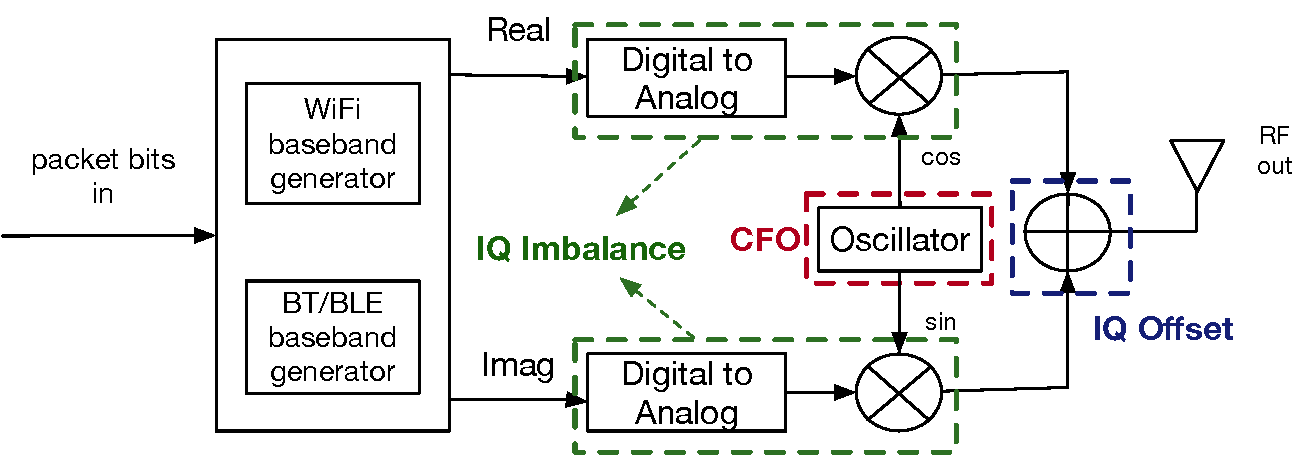
\includegraphics[width = \linewidth]{bletracking/plots/IQchain.pdf} 
    \caption{Architecture of WiFi/BLE combo chipsets}
    \label{fig:iq_arch}
\end{figure}

A consequence of this hardware design choice is that BLE transmissions contain the
same hardware imperfections as WiFi. The imperfections are introduced by the
shared I/Q frontend of the chipset (Figure~\ref{fig:iq_arch}). They result in
two measurable metrics in BLE and WiFi transmissions: \emph{Carrier Frequency
Offset (CFO)} and \emph{\iq imperfections}, specifically: \iq offset and \iq
imbalance.  Prior work demonstrated that these metrics are sufficient to
uniquely fingerprint WiFi devices~\cite{Brik_radiometric}.
The following describes how each of these metrics are calculated and how 
they result from manufacturing variations:


\subsubsection*{CFO} It is an offset in the carrier frequency
generated by the RF frontend's local oscillator. The carrier frequency is
ideally exactly the center frequency of the channel in use. However,
imperfections in the radio's local oscillator, a crystal oscillator, yields a
unique CFO added to every transmission.  Crystals cut in different ways yield
different tolerances in how much an individual crystal's frequency can deviate
from the true value it was to produce for. This imperfection manifests as CFO
because the local oscillator is mixed with the baseband signal (e.g., WiFi or
BLE) in the RF frontend, so it can be transmitted; thereby, carrying the
crystal's imperfection as a feature in the transmission.

\subsubsection*{\iq imperfections} These are a result of the following two
phenomena. \emph{\iq Offset} is created by two different imperfections in the RF frontend: (1) the
carrier frequency signal leaking through the mixer into the transmitted signal,
or (2) the baseband signal having a DC offset. \iq offset results in a fixed
complex term added to each received \iq sample (i.e., a shift in the center of
the constellation). \emph{\iq Imbalance} occurs because of a mismatch between
the parallel analog components of the RF chain in I (in-phase) and Q
(quadrature) signal paths. This results in asymmetry in the phase and amplitude
of received \iq samples.

\subsection{BLE is more difficult to fingerprint than WiFi}
\label{sec:methodology:diff}

\begin{figure}
    \centering
    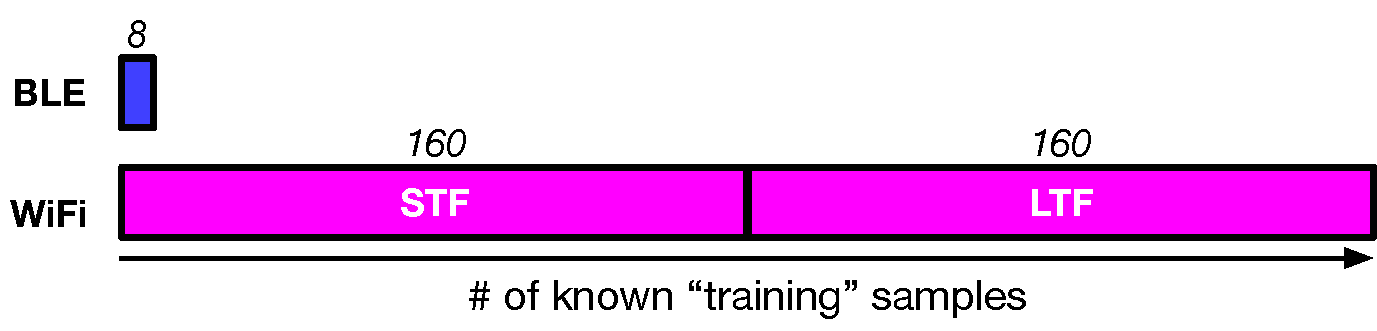
\includegraphics[width=\linewidth]{bletracking/plots/knownsamples}
    \caption{
      Length of known samples in BLE and WiFi packets.
    \label{fig:training_length}
  }
\end{figure}

Measuring transmitter imperfections is significantly more challenging for BLE
transmissions than it is for WiFi transmissions.
%
The problem is, BLE signals are Gaussian Frequency Shift Keying
(GFSK) waveforms that do not require accurately correcting CFO and \iq imperfections
for decoding. 
%
Conversely, WiFi signals are wideband multi-carrier waveforms, therefore their
decoding algorithm requires accurately correcting for CFO and \iq imperfections for decoding.

As a result of this issue, BLE packets contain fewer
known ``training'' samples used for measuring imperfections than WiFi
(Figure~\ref{fig:training_length}). BLE packets have only 8 training samples,
while WiFi packets have 320 training samples.
%
BLE receivers use these symbols to implement very coarse grained CFO correction.
%
Namely, they average the two frequencies (symmetric positive and negative
frequencies are used to represent 0 and 1 symbols) in BLE's training
sequence to produce a coarse grained average CFO~\cite{cvtracksun}.
%
%Since the preamble is an 8-bit sequence of consecutive 0 and 1, the frequency
%of preamble is symmetric.  Therefore, ideally the average of the frequencies
%in preamble must be 0. If there exists CFO, this average will be an estimate
%of CFO.
%
%These CFO estimates are coarse grained because they only rely on 8 samples in the preamble.
%Consequently, they do not produce an accurate estimate of CFO---leading to
%confusions between device fingerprints.
%
Indeed, with only 8 samples at BLE's 1~MHz sample rate, the theoretical limit of CFO accuracy is 2~kHz
assuming 3 degree phase noise, even at high SNR (40 dB). 

To make matters worse, inaccurate coarse compensation of CFO significantly affects our ability to measure \iq imperfections. Inaccurately compensating CFO will result in time-dependent phase shift distorting the \iq constellation, making it challenging to accurately estimate \iq imperfections.

Prior fingerprinting techniques developed for other protocols are not capable of overcoming these challenges.
%: short preamble and/or lacking structure for CFO estimation. 
Therefore, prior approaches can not be used to fingerprint BLE~\cite{vohuuusrp,Brik_radiometric,deviceID_kose,Intrusion_hall,suskitransient,deeplearning_merchant,lora_robyns,gopalakrishnan2019robust}.
%\subsubsection{Why not use neural networks?}

Another approach to fingerprinting BLE transmissions would be to use neural networks. 
Although neural networks can address these challenges, we did not use them in
this work because of the following limitations: (1) 
Neural networks make it difficult to determine
the significance and distinguishably of each type of hardware imperfection
(e.g., CFO, \iq offset), (2) Neural networks also can overfit to a specific
bit pattern in a packet, rather than the transmitter imperfections. This is problematic because
BLE advertisements do not have a stable bit pattern: MAC addresses change every
15 minutes.  (3) In our preliminary experiments with neural nets, 
we found they require significantly more training data than the conventional
classification we describe in this work.

\subsection{Accurate measurement of BLE's CFO \& I/Q imperfections} %{{{
\label{sec:methodology1}


% \subsubsection*{Comparison with other fingerprinting methods}

%
%The reason is, BLE is an extremely low-energy protocol: BLE's physical-layer
%signal is designed to require simple hardware to transmit and receive messages.
% 

% BLE signals are generated by representing the bits as basic  Gaussian Frequency Shift Keying (GFSK) modulation, where $f_0$ means bit $0$ and $f_1$ means bit $1$. 
% Although symbols in a BLE signal are not modulated in I/Q domain, often the CFO and IQ imperfections are embedded in the BLE signals as a part of the transmitting them from an I/Q modulator based radio. Ideally, an attacker would need to receive these samples, and extract these 
% impariment using the simple FSK signal. The standard BLE receivers can decode the 
% packet without explicity correcting for CFO or IQ imperfections as FSK is a non-IQ modulation scheme. 
% There are two key challenges with extracting CFO and IQ imperfections:




\begin{figure}
    \centering
    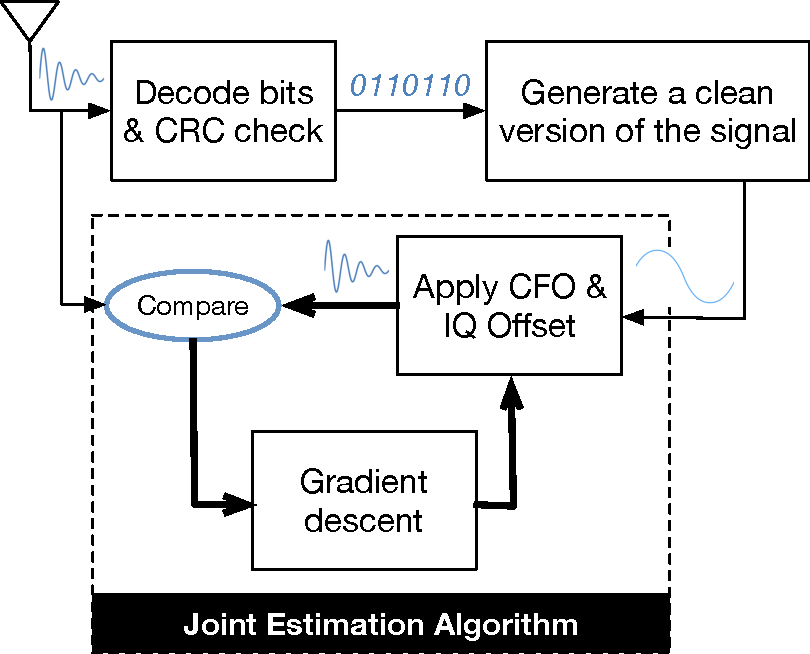
\includegraphics[width = 0.75\linewidth]{bletracking/plots/jointestimation.pdf} 
    \caption{Our new BLE imperfection estimation method.}
    \label{fig:overview}
\end{figure}

\begin{comment}
We demonstrate it is possible to accurately estimate CFO and I/Q
imperfections of BLE signals by overcoming the primary challenges of
BLE fingerprinting with a novel fingerprinting technique
(outlined in Figure 3). First, to overcome the challenge of measuring
I/Q imperfections requires accurately measuring CFO, we
present a novel approach that jointly estimates CFO and I/Q
imperfections. Second, to accurately estimate CFO and I/Q
imperfections with only BLE's short known training symbol
sequence, we decode the entire received BLE packet and
reconstruct a clean BLE waveform (only when the CRC check
passed). Therefore, instead of relying on the 8 known samples
in the preamble, we can utilize the entire packet ($\sim$ 370
samples). These additional samples provide a theoretical CFO
measurement precision of about 40 Hz compared to 2 KHz
from coarse-grained estimation.
Then, we leverage the clean reconstructed BLE waveform and distort it with varying CFO and I/Q imperfections. We do so until we find CFO and I/Q estimates such that the reconstructed signal matches the original received signal (as shown in Fig.~\ref{fig:overview}).
Brute force search for these hardware imperfection parameters
would incur a significant computational cost because search space for these imperfection parameters is
vast. As a result, we use optimization techniques to efficiently
move towards the optimal parameters where the distorted reconstructed signal matches the received signal.
\end{comment}
The fingerprinting methodology we present in this work (Figure~\ref{fig:overview}) is the first
physical-layer identification method that can accurately estimate CFO and I/Q
imperfections of BLE signals. To fingerprint BLE, we need to overcome the following two fundamental
challenges:

Accurate estimation of CFO (and \iq imperfections) is not feasible with BLE's short 
training symbol sequence (preamble). Instead of
relying on the 8 known samples, we can utilize the entire
packet ($\sim$370 samples). This results in a theoretical CFO
measurement precision of about 40~Hz compared to 2~kHz from BLE's coarse CFO estimation. 
%
The next question is: how can we leverage the entire decoded packet to estimate 
CFO and \iq imperfections accurately?

First, we decode the entire received BLE packet (for packets with a valid CRC) and reconstruct a
clean BLE waveform (Figure~\ref{fig:overview} top).
Then, we leverage the clean reconstructed BLE waveform and distort it iteratively, 
%
we do so until we find CFO and \iq imperfection estimates where the %re-encoded
reconstructed
signal matches the original received signal (Figure~\ref{fig:overview} bottom). 
Brute force search for the optimal CFO and \iq imperfections 
requires significant computational complexity because we need
to search all possible values.
We use optimization techniques to make this more efficient.
The primary insight of our optimization approach is as follows: estimating \iq imperfections of a received signal depends on the estimates of the signal's CFO.
Therefore, as we get closer to an accurate estimate of CFO, we reduce the search space to find accurate \iq imperfections. We build on this insight
%To make this estimation efficient, our insight is \iq imperfections are dependent on estimates of CFO.
 and present a joint CFO and \iq imperfection estimation methodology.
 % enabling us to use optimization techniques to efficiently find the matching parameters.

%Now that we can theoretically get 40~Hz, 

%To overcome the issue, we 
%

%\subsubsection*{Challenge 2. \iq imperfections depend on CFO estimation}

% TODO HOME
%Accurate \iq imperfection estimation requires accurate CFO estimation.
%Therefore, we can not estimate CFO and \iq imperfections separately. To resolve this, we present a novel
%approach that jointly estimates CFO and I/Q imperfections.   


\subsubsection*{Jointly estimating CFO and I/Q}

Let $y$ be the captured complex baseband BLE signal (normalized by the average amplitude). In a GFSK modulated signal, ideally we have $Real\{y\} = cos(\omega(t)t)$ and $Imag\{x\} = sin(\omega(t)t)$ where $\omega(t)$ is the baseband frequency of the signal which is generated according to the GFSK modulation. However, the presence of hardware imperfections will slightly change the baseband signal. We first decode the signal to obtain the sequence of bits and then, we make $\omega(t)$ according to GFSK modulation. Let $y'$ be the model of the imperfect signal. With the effects of CFO and \iq imperfections, the baseband signal becomes:

\begin{gather*}
    y'(t) = A \times \big[(1-\frac{\epsilon}{2})cos(\omega(t)t-\frac{\phi}{2})+I+ \\
    j\big((1+\frac{\epsilon}{2})sin(\omega(t)t+\frac{\phi}{2})+Q\big)\big] \times e^{j(\phi_o+2\pi f_o t)}
\end{gather*}
where $f_o$, $\phi_o$, $A$, $\frac{1-\epsilon}{1+\epsilon}$, $\phi$, $I$ and $Q$ denote CFO, phase offset, normalized amplitude of the signal, \iq amplitude imbalance, \iq phase imbalance, I offset and Q offset, respectively. The goal is to choose the value of these variables in such a way that $||y'-y||^2$ is minimum and as a result, $y'$ is as close as possible to the captured signal $y$. Therefore, we must solve the following optimization problem:
\begin{gather*}
    min_{f_o,\phi_o,A,\epsilon,\phi,I,Q}{F=||y'-y||^2 =} \\ |Real\{y'\}-Real\{y\}|^2+|Imag\{y'\}-Imag\{y\}|^2
\end{gather*}

\begin{figure}
    \centering
    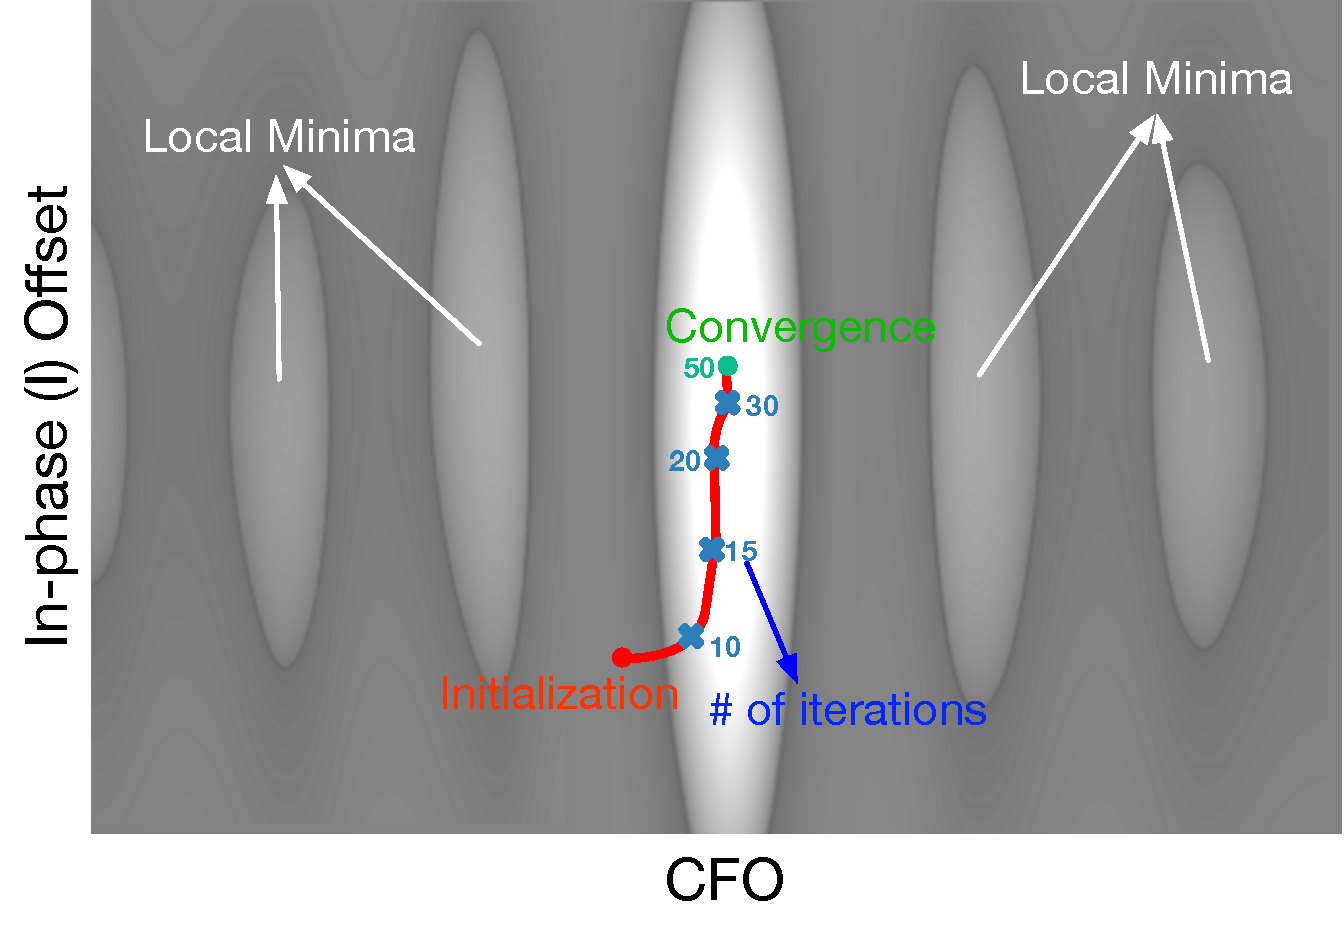
\includegraphics[width=0.9\linewidth]{bletracking/plots/algo_heatmap.pdf} 
    \caption{Process of jointly estimating CFO and \iq offset.}
    \label{fig:heatmap}
\end{figure}

However, this problem is not convex, and the objective function has several local minima (Figure~\ref{fig:heatmap}). To avoid optimization techniques ending up in a local minimum, we initialize the variables properly. This increases the chance of finding the global minimum. Although theoretically we aren't guaranteed to reach the global minimum for arbitrary optimum numbers of these variables, we found in practice the initialization helps us reach the optimum value.

To initialize CFO, we start by taking the average of frequencies in the preamble. Then we compensate the initial CFO in the signal to get the signal $z = y e^{-2\pi f_o t}$. To estimate initial \iq imperfections, we use the \iq constellation of the GFSK signal. The \iq constellation of an ideal GFSK signal is a circle centered at $(0,0)$. However, \iq imperfection will change this constellation. Specifically, \iq offset shifts the center of the constellation, and \iq imbalance changes the shape from a circle to a tilted ellipse.
%
%These effects are shown in Figure~\ref{fig:iq_const}.
As a result, to get an initial estimation of \iq imperfections, we fit an ellipse to the 2-dimensional points $(Imag\{z\},Real\{z\})$ by minimizing the Least Square Error. The center of the ellipse will provide the initial \iq offset, and initial \iq imbalance can be obtained from the ratio of minor and major diameter and rotation angle of the ellipse.

\if 0
\begin{figure}
    \centering
    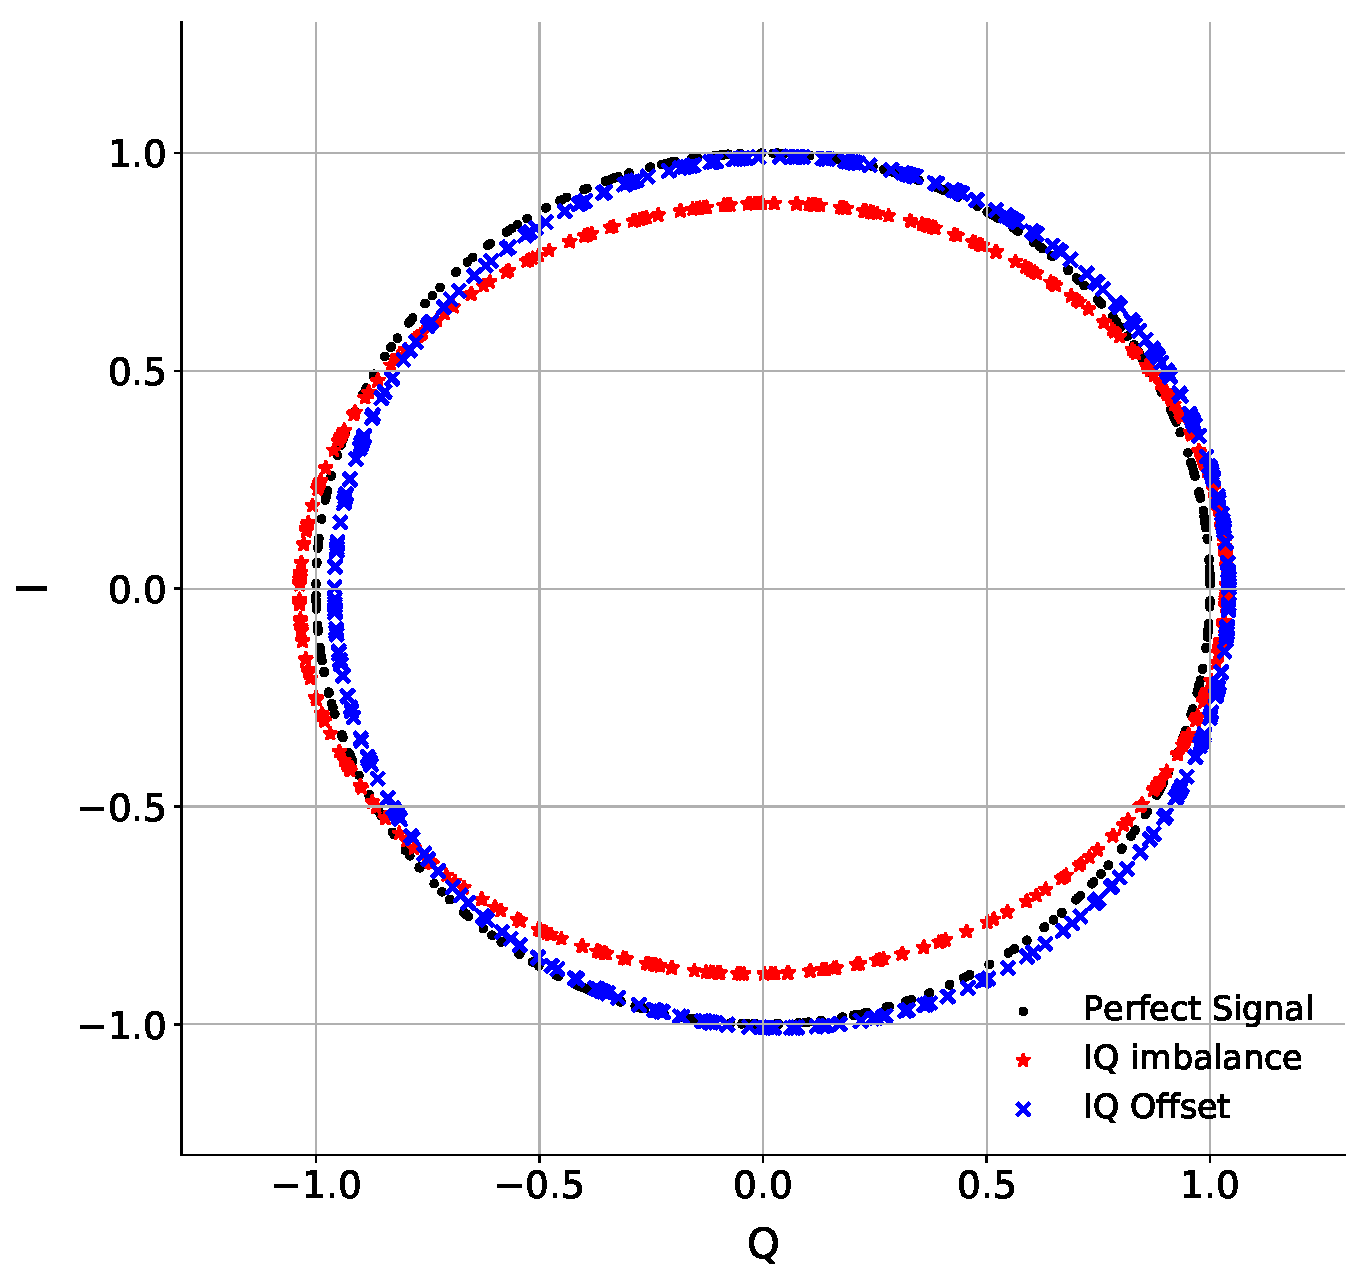
\includegraphics[width = \linewidth]{bletracking/plots/IQ_const.pdf} 
    \caption{Effects of IQ imperfection on IQ constellation of a GFSK signal without noise and CFO}
    \label{fig:iq_const}
\end{figure}
%it will be long if I want to explain this ellipse thing
\fi

Although these initial estimations are close to optimum,
they are not accurate. 
%
As mentioned earlier, this CFO initialization is based on an 8~symbol preamble and therefore not accurate. 
%
Moreover, an inaccurate CFO estimate will cause a time-dependent phase
shift which distorts the \iq constellation. 
%
Therefore, the initial \iq offset
and imbalance estimation will also have errors. 
%
Consequently, we employ
optimization techniques to jointly estimate these imperfections using the initial estimates. 
 
%However, finding these optimal values can be extremely computationally expensive. 
%
%Indeed, the naive approach would be to brute force all possible values for CFO, \iq offset and \iq imbalance to find the optimal values. 
%
We chose gradient descent to solve the optimization problem, as it ensures that we move towards the optimal values after each step. 
%
Specifically, we use a quick form of gradient descent, Nesterov Accelerated Gradient Descent (NAG) to move from the initialization towards the optimum values
of $f_o,\phi_o,A,\epsilon,\phi,I,Q$ by minimizing $F$ in the mentioned
optimization problem. 
%
NAG adaptively adjusts the parameter update at each step, so that we move faster towards the optimal value at the start but slow down as we get close to the minima.

\begin{comment}
Therefore, after this initialization, we use Nesterov
Accelerated Gradient Descent (NAG) to move from the initialization towards the optimum values
of $f_o,\phi_o,A,\epsilon,\phi,I,Q$ by minimizing $F$ in the mentioned
optimization problem. 
\end{comment}


Figure~\ref{fig:heatmap} demonstrates the process of how we start from the initial estimations of CFO and \iq imperfections, then move toward the optimal values of CFO and \iq imperfections using gradient descent (the red line), and finally converge to the accurate estimations of CFO and \iq imperfections in a few iterations. Since this optimization problem is not convex, it is still possible we end up converging to a local optima. Therefore, if after convergence, the average of $F$ was not less than a certain threshold (determined according to SNR), we adjust the initialization values by a fixed step and repeat the gradient descent process. 

% TOO LONG ====================
%However, as mentioned earlier, this optimization problem is convex and we may converge to the local optima. Therefore, if after convergence, the average of $F$ was not less than a certain threshold which is determined according to SNR, we add certain steps to the first initialization and repeat the aforementioned gradients descent process. We keep searching for the optimum with new initializations until either the average of $F$ falls below the threshold or our initialization falls out of the bound of the typical values for these imperfections (in which case we give up on the packet. This typically happens when the SNR is less than 5 dB or there is a collision). The first initialization will increase the speed of convergence as usually it will be close to the optimum and re-initialization will ensure ending up in a point which is either the global optimum or very close to global optimum (in the sense that the objective function is less than the desired threshold and hence, is within a small margin of global optimum). The proposed algorithm fulfills the two key properties that we explained at the beginning of this subsection. First, the NAG based joint estimation of CFO and IQ imperfections ensures precise estimation with fine granularity as it keeps moving towards the optimum with adaptive steps and removes the mutual effect of mismatch in estimating these imperfection parameters. Second, the objective function of optimization is chosen as the summation of all PHY samples across the packet, which diminishes the impact of AWGN and provide more robust information and granularity. The final result is achievement of a highly precise CFO and IQ estimates for a device, that are robust to environmental noise, and can therefore be used by an attacker as a unique fingerprint for generic consumer devices.
% Shorter ==========

The proposed optimization based estimation ensures accurate estimation with fine granularity as it keeps moving towards the optimum with adaptive steps and removes the mutual effect of mismatch in estimating these imperfection parameters. Moreover, the objective function of the optimization is chosen as the summation of all samples across the packet, which diminishes the impact of the channel and provides fine-grained estimates of the CFO and \iq imperfections.

% This is restated, so cutting other eval is there now
\if 0
We use this methods to extract CFO, IQ offset and IQ imbalance for 20 ESP32 chipsets of the same make and model. Figure~\ref{fig:esp} represents CFO and IQ offset magnitude for 10 packets for each of these 20 chipsets. The low variance of CFO for each device, shows these methods is very accurate in measuring hardware imperfections (e.g. the CFO standard deviation average for 20 devices is 200 Hz in our algorithm which is significantly less than the existing methods described earlier). Obviously, low within-device variance will significantly improve the identification accuracy and these 20 devices can be clearly distinguished only by their CFO and IQ offset. 
\fi

%\vspace{0.5em}
%\noindent\textbf{Comparing CFO accuracy} %{{{
%
\subsubsection*{Evaluating CFO estimation accuracy}
To evaluate the accuracy of our new fine-grained fingerprinting algorithm compared with BLE’s default coarse
CFO estimation, 
we compute the standard deviation of CFO measured for 100 packets from each device in a set of 100 different BLE transmitters observed in the field. % For each device, we
%consider the CFO estimation technique which yielded the lowest standard deviation (std).
%
 Figure~\ref{fig:cfo_comp} shows the CDF of the standard deviation of the CFO across all transmitters, for both techniques.
%
We see that 
our fine-grained CFO estimation significantly reduces the standard deviation of CFO estimation for all devices. This reduces the within-device variance, making fingerprints easier to distinguish.
%Moreover, as inaccurate estimation and compensation of
%CFO affects the estimation of IQ imperfections since the residual CFO will
%cause IQ samples to rotate by time.
% In fact, no prior work has
%demonstrated that it is possible to obtain accurate and identifiable estimates
%of imperfections for BLE transmitters.
%
%Consequently, we must develop a new
%algorithm to enable find-grained and robust estimation of CFO and IQ
%imperfections to enable our device identification attack.

%The resulting standard deviation of the measured CFO was 1.5 KHz (we averaged the CFO standard deviation across 20 different devices). This standard deviation is huge for performing the task of RF fingeprinting and will end up in low accuracy of identifying devices based on RF fingerprints. 
%}}}
\begin{figure}
    \centering
    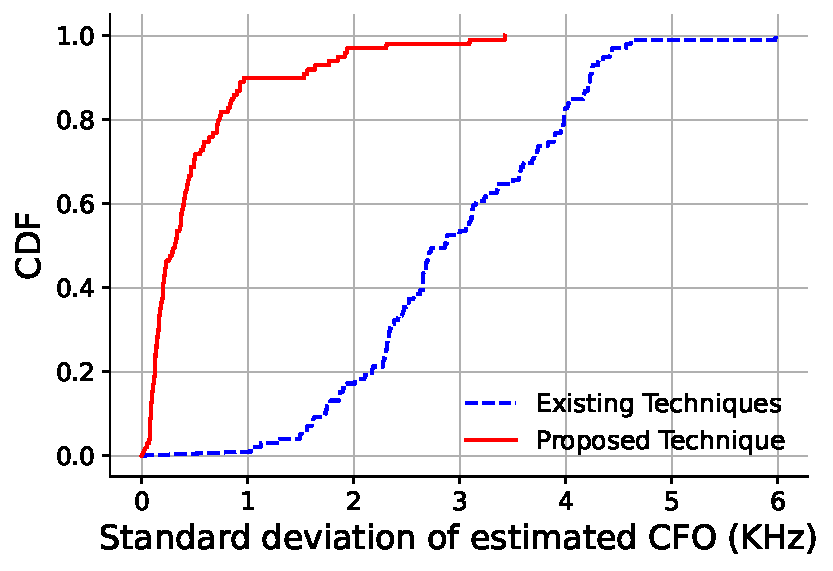
\includegraphics[width = \linewidth]{bletracking/plots/CFO_comparison_ESP2.pdf} 
    \caption{Comparing the CFO estimation of existing coarse-grained techniques with our proposed technique.}
    \label{fig:cfo_comp}
\end{figure}


%\vspace{0.5em}
%\noindent\textbf{Summary:} 
\subsubsection*{Summary}

We demonstrate that it is feasible to estimate CFO and \iq
imperfections of WiFi/BLE combo chipsets accurately; even
though BLE does not have the rich signal features that are
present in WiFi.

\subsection{Fingerprinting and identifying a target device}
\label{sec:methodology2}
With fine-grained estimates of the CFO and \iq imperfections in BLE transmissions, we can now execute a BLE location tracking attack.
The first step in the attack is capturing BLE packets. We use an SDR to capture raw I and Q samples of nearby BLE transmissions. %Next, we use the captured signal to fingerprint the target device.
The captured BLE packets are processed in two stages---fingerprinting and identification. In the fingerprinting stage the target device is briefly isolated, and we capture a number of packets that we use for building a fingerprint for the device (i.e., training packets). The latter stage identifies if a captured BLE packet matches the fingerprint of the target device.

%\vspace{0.5em}
%\noindent\textbf{Fingerprinting Stage:} 
\subsubsection*{Fingerprinting Stage}
For each packet from a device $D$, we extract CFO and \iq imperfections using the algorithm described in~\ref{sec:methodology1}. Let $x_1,...,x_N$ be the CFO and \iq imperfection feature vectors for $N$ training packets we have received from device $D$. We calculate the mean $\mu_D$ and covariance matrix $\Sigma_D$ of $X = [x_1 \quad ... \quad x_N]$. $\mu_D$ and $\Sigma_D$ together with a threshold that will be defined later is considered the profile of device $D$.

%\noindent\textbf{Identification Stage:} 
\subsubsection*{Identification Stage}
In identification stage, we want to decide whether a packet $x_t$ was transmitted by device $D$, indicating that the target device is near the SDR. To do so, we compute the Mahalanobis distance to the profile of device $D$:

\begin{gather*}
    distance(x_t,\mu_D,\Sigma_D) = \sqrt{(x_t-\mu_D)^T\Sigma_D^{-1}(x_t-\mu_D)}
\end{gather*}

This distance metric measures how close the features of the new packet are to the profile of device $D$. In addition to $\mu_D$ and $\Sigma_D$, we define a threshold $thresh$ as the profile of the device. Whenever $distance(x_t,\mu_D,\Sigma_D)<thresh$ for packet $x_t$, we identify the packet as being transmitted by the target device $D$. The threshold can be chosen in two ways. One way would be to choose a threshold that guarantees a certain FNR in a validation set. Another way can be to pick a threshold that minimizes $FPR^2+FNR^2$, so that their values are balanced. In this paper, we use these two methods for selecting the threshold depending on the goal of the experiment.

Additionally, since the MAC address of every BLE device is stable for a limited duration of time, we can receive multiple packets that we know belong to the same BLE device. As a result, we can use multiple packets to identify a BLE device, reducing inter-packet noise. One way that we found most effective to use multiple packets was to first average the feature vector $x$ for all packets from the same BLE device, and then compute the Mahalanobis distance. This averaging reduces the effect of small deviations in the imperfections across packets.

\subsubsection*{Summary} We identify a device based on the Mahalanobis distance to its previously recorded hardware imperfection fingerprint. Also, since BLE devices have temporarily stable identifiers in their packets, we can identify a device based on the average over multiple packets, increasing identification accuracy.

\if 0 % extra {{{
\paragraph{Fingerprinting Stage} For each packet from a device $D$, CFO and IQ imperfections (IQ offset and IQ imbalance) can be extracted with a high resolution using algorithm described in~\ref{sec:methodology1}. Let $x_1,...,x_N$ be the CFO and IQ imperfection feature vectors for $N$ training packets we have received from device $D$. We calculate the mean $\mu_D$ and covariance matrix $\Sigma_D$ of $X = [x_1 \quad ... \quad x_N]$. $\mu_D$ and $\Sigma_D$ together with a threshold that will be defined later is considered as the profile of device $D$.



%Note that IQ offset and imbalance are only useful for combo transmitters and will be ignored by classifier while classifying BLE-only transmitters.
\paragraph{Identification Stage} In identification stage, we want to decide whether a packet $x_t$ with a new MAC address belongs to device $D$, indicating that the target device is present. To do so, we compute the Mahalanobis distance to the profile of device $D$

\begin{gather*}
    distance(x_t,\mu_D,\Sigma_D) = \sqrt{(x_t-\mu_D)^T\Sigma_D^{-1}(x_t-\mu_D)}
\end{gather*}
\begin{gather*}
    distance(x_t,\mu_D,\Sigma_D) = \sqrt{(x_t-\mu_D)^T\Sigma_D^{-1}(x_t-\mu_D)}
\end{gather*}
%This is assuming that the estimated CFO and IQ imperfections have a Gaussian distribution which is a fair assumption considering that the tolerance in CFO and IQ imperfection estimation of a device for different packets is mainly caused by variations in SNR (which affects estimation error) and tolerance of the underlying hardwar.
This distance is one way to measure how close the features of the new packet are to the profile of device $D$. In addition to $\mu_D$ and $\Sigma_D$, we define a threshold $thresh$ as the profile of the device. Whenever $distance(x_t,\mu_D,\Sigma_D)<thresh$, packet $x_t$ belongs to the target device $D$ and device $D$ is identified. Otherwise, packet $x_t$ belongs to some other device in the world that we are not looking for. This threshold is chosen by using the validation set.
Moreover, since the MAC address is fixed for a period of time, we receive a number of packets with the same MAC address which we know belong to the same device. As a result, we can make a decision about the identity of the MAC address instead of the individual packets. One way that we found most effective, was to first average the feature vector $x$ for all packets with the same MAC address and then compute the Mahalanobis distance. This would further reduce the tolerance due to estimation error and inherent tolerance of features.


\fi
%}}}



